%\input{chap1/introduction.tex}

\setcounter{chapter}{0}

\chapter{Introduction}\label{sec:intro}
In this chapter, we introduce the context of this research, which is about communities of web services abstracted as autonomous agents. Those agent-based web services use intelligent decision making mechanisms to improve their performance in multi-agent setting. We discuss the motivations of this work and briefly review the literature to identify the problems we aim to solve in this thesis. Moreover, we discuss our objectives and contributions.

\section{Context of Research}\label{sec:motivation}

Over the past years, online services have become part of many
scalable business applications. The increasing reliance on
web-based applications has significantly influenced the way web
services are engineered. Web services provide a set of online software functions accessible at a network address over the web.
The recent developments are shifting web services from passive and
individual components to autonomous and group-based components
where interaction, composition, and cooperation are the key
challenges \cite{ICWS2011-1,SCC2011-1}. The main objective is to
achieve a seamless integration of business processes, applications
and web services. Delivering high quality services considering the
dynamic and unpredictable nature of the Internet is still a very
critical and challenging issue.

Typically, web services are business applications deployed as
autonomous and interoperable agents \cite{Alescio}. In fact, the
W3C consortium defines a web service as ``an abstract notion that
must be implemented by a concrete agent''. However, the web is
stocked with agent-based services that offer similar business
functionalities, which leads to service consumers having
difficulties in choosing the most appropriate agents to interact
with.

The need for highly available and responsive services has called
for grouping and collaborative mechanisms of loosely-coupled web
services, particularly in business settings. The idea of grouping
web services within communities and the way those communities are
engineered so that web services can better collaborate have been
proposed and investigated in
\cite{DBLP:journals/ijebr/MaamarSTBB09,DBLP:journals/internet/BenatallahSD03,Rosario:2008:PQS:1512146.1512290}.
Communities are virtual groups of web services having similar
functionalities \cite{Zeng:2003:QDW:775152.775211,
Paik:2005:TSS:2229263.2230038,Medjahed05adynamic,10.1109/ARES.2008.7},
but probably different non-functional quality attributes, which
form the QoS parameters.
%When communities are used, users send
%their requests to the masters of those communities, which are
%responsible of managing the communities, forwarding the requests
%to the suitable member web services and checking the credentials
%of those members.
Communities aim to provide higher service
availability and performance than what individual web services can
provide.
%The high availability of services and the community
%resilience to failure are guaranteed since web services can
%cooperate and replace each other within the same community and
%since there is no single point of failure in the communities
%architecture.

\section{Motivating Scenario}\label{sec:motexample}

In this section, we present a scenario and demonstrate why there
is need for communities of services. We first propose an example
of a real world scenario, focusing on user experience. There are a
plethora of options available to people in today's society,
including weather forecasting, ticketing services, map services,
local places guides and so on. Most mobile or web applications
cannot independently satisfy users requests and should rely on
different online services. The high competition within the
services industry requires applications to use reliable and high
quality online services.


If the user were to check a web site or run an application on her
mobile device upon having downtime, or having high response delay
or encountering any non-satisfying quality metric, she will
instantly remove the application, which is a huge business concern
for application providers. For example, if a user installs a
ticketing application on her mobile device and the application is
not using high quality service providers, the user would instantly
uninstall the application, which has an extremely negative impact
on the
visibility of the application. %Let us say you search "Montreal
%Weather" on a search engine and you click on a web site which is
%slow because it is using a bad weather web service as source of
%its raw data, the user will leave the web site and try another
%link from search results, which has a bad Search Engine
%Optimization (SEO) effect for the web site, and search engines
%would not show that web site on search results anymore, which is a
%business and revenue loss for the application.
Thus, end user satisfaction is the main goal for competitive
online providers. Communities of web service, by providing
services with higher quality, higher uptime and reliability for
end users, aim to reach this goal. To this end, community
management decisions should capitalize on important QoS parameters
while forming the community and during membership management.


High demand on online services has created a massive business
competition. For example, nowadays users are provided with
multiple choices of web services offering local places information
such as coffees, venues, and shops nearby a geographic position.
It is hard for new web services to find their customers and be
visible for end users amongst hundreds or thousands of other
available services, even if they provide a high quality of
service. Hence, the concept of communities of web services
provides them with the chance of joining a platform with an
established market share and reputation. However, it is crucial
for a community manager to consider many factors when inviting or
accepting new members. For example, if the market share is not big
enough, bringing new web services can cause revenue drop for the
already residing members. This may encourage other web services to
collude, leave, or join other communities, hurting the community
stability. This is an important issue which has not been addressed
previously in the relevant literature. On the other hand, if
communities bound the number of web services to ensure higher
revenue, availability and response time could be negatively
affected if some members encounter problems. This is because
alternative web services for substitution will be limited.  This
has also not been efficiently addressed in the related work.
Consequently, community formation algorithms satisfying some
desirable properties such as community stability and overall
revenue are yet to be defined considering end users, community
managers and service providers.


\section{Motivation and Research Questions}\label{sec:researchquestions}

Web service communities are dynamic by design
\cite{DBLP:journals/ijebr/MaamarSTBB09}. In these communities, web
services are modeled as intelligent autonomous agents, where they
can adopt a strategy maximizing their payoff at any time. A web
service can ask joining a community and has the right to leave it.
Community managers can invite or ask a web service to leave in
order to maximize the community profit. Users can simply stop
sending requests to a web service which is not providing
satisfactory services. Thus, it is important to consider all the
parties involved in the decision making process about the
community formation and management. Most of the recent work on communities of
services are either user-centric and focus on user satisfaction
\cite{Chun02user-centricperformance} or system-centric and focus
on the whole system throughput, performance and utilization. There
are many contributions in distributed, grid, cluster and cloud
services which are system-centric. However, in real world
environments and applications, both users and service providers
are self-interested agents, aiming to maximize their own profit.
In those environments, both parties (users and services) will
collaborate as long as they are getting more benefits and payoff.
Our initial research question is: \emph{How can we model the
community of agent-based services in order to maximize the utility
of involved users, web services and community organizers? [R1]}


In order to address this problem, recently
\cite{DBLP:conf/IEEEscc/LimTMB12,
DBLP:conf/IEEEscc/KhosravifarABT11, 10.1109/TSC.2012.12} proposed
mechanisms to help users and services maximize their gain. A
two-player non-cooperative game between web services and community master (i.e., manager) was introduced in
\cite{DBLP:conf/IEEEscc/KhosravifarABT11}. In
\cite{DBLP:conf/IEEEscc/LimTMB12}, a 3-way satisfaction approach
for selecting web services has been proposed. In this approach,
the authors proposed a web service selection process that the
community masters can use. The approach considers the efficiency
of all the three involved parties, namely users, web services and
communities. The issue with these solution concepts is that they
consider community as a whole and model it as one entity in their
formulations. A community master decides on behalf of all the
members using an aggregated function of parameters. This can hurt
the overall revenue for some individual web services, or even a
subset of web services. Those services can collude and form their
own community to increase their payoff, instead of having to adjust and share
their resources with other members. Another important issue which
needs to be considered is the community stability. In community of
web services, the members and community organizers collaborate to
perform tasks. Having jointly completed a task and generated
revenue, they need to agree on some reasonable method of dividing
profits (or tasks) among themselves. This is a key issue for the
group stability still to be investigated. If the revenue sharing
mechanism is not fair enough for any subset of web services
working in the community, these agents, as profit maximizing
entities, would deviate and make their own group. Thus, an important an
important research question that we would like to address is:
\emph{How can we model fair and stable communities as coalitions
of agent-based web services? [R2]}

%The consideration of those inputs is a significant
%issue as existing web services can lose utility or payoff because
%of the new member, which can results in an unhealthy and unstable
%group. The problem comes from the fact that the existing members
%should collaborate with the new web services, so probably their
%performance as a group can suffer. Existing members may even
%deviate and try to join other communities if they are unsatisfied.
%Those considerations of forming stable and efficient coalitions
%are the main contributions of our paper.

%However, a high
%performing web service could deviate anytime it finds itself
%unsatisfied within the community instead of adjusting its service
%parameters.


In \cite{10.1109/TSC.2012.12}, a cooperative scheme among
autonomous web services based on coalitional game theory has been
introduced. The authors have proposed an algorithm to reach
individually stable coalition partition for web services in order
to maximize their efficiency. The communities choose new web
services on the promise that it would benefit the community
without decreasing any other web service's income. In their model,
the worth of community is evaluated with high emphasis on the
availability metric and considering price and cost values only.
The community structure is based on a coordination chain, where a
web service is assigned as a \emph{primary} web service and the
community task distribution method will initially invoke the
primary web service. Only if the primary web service is
unavailable, the next backup web services in the ordered
coordination chain will be invoked. However, in cooperative
models, it is preferred to have a real and active cooperative
activity engaging all agents to perform the tasks more
efficiently. Thus, the final research question we aim to investigate is: \emph{How can we model and analyze the cooperation
among the community members in realistic, applicable and practical
settings? [R3]}

Within communities, services can exhibit competitive behavior as they provide the same functionalities and the number of users requests is finite.
However, for the same reason of being functionally similar, services can cooperate with each other, for example to substitute each other in order to perform some sub-tasks.
For instance, services can opt for performing tasks if they feel they are capable enough
or decide to cooperate by showing the availability to perform some sub-tasks. The relevant question to be addressed is: \emph{How can we design a community model where both competitive and cooperative behaviors exist? [R4]}

In most of the recent work on communities of web service, the solutions consider the architecture of centralized management for communities where most of the decisions are made by the centralized coordinator. However, in real world scenarios, decisions made by independent service providers are highly distributed.  \emph{How can we model a distributed decision making process for the problem of forming communities of services? [R5]}

Also in all of the mentioned proposals, the community manager as a centralized entity, has complete information of all the web services and their quality. However, centrality and complete information are strong assumptions, which are not fully compatible with real business scenarios.
\emph{How can we train web services based on limited information to operate efficiently? [R6]}

% ooooooold
%\indent When monitoring a dialogue between two or more agents, there are many question that should be answered. In this thesis, we are interested in answering the following questions:
%\begin{itemize}
%\item How much are agents certain about selecting a move at each dialogue step?
%\item How much are agents certain about their dialogues?
%\item How good are agents in the real dialogue (i.e. the effective dialogue)?
%\item How far are agents from the right dialogue (i.e. the best dialogue given the knowledge bases of the participants)?
%\end{itemize}
%Answering these questions is undoubtedly complex. Therefore, we do not expect a comprehensive answer to all these questions.

\section{Contributions}\label{sec:motexample}

\subsection{Contribution 1: Efficient Coalition Formation for Web Services} 

%\cite{10.1109/TSC.2014.2312940}.}

In this research work\footnote{This contribution was published in \cite{10.1109/TSC.2014.2312940}}, our first objective is to propose a
cooperative model as game for the aggregation of web services
within communities. The solution concepts of our cooperative game
seeks to find efficient ways of forming coalitions (teams) of web
services so that they can maximize their gain and payoff, and
distribute the gain in a fair way among all the member services.
Achieving fairness when the gain is distributed among the
community members is the main factor to keep the coalition stable
as no web service will expect to gain better by deviating from the
community. In other words, the coalition is made efficient if all
the members are satisfied. We first propose a representation
function for communities of web services based on their QoS
attributes. By using this function, we can evaluate the $worth$ of
each community of web services. When facing new membership
requests, a typical community master checks whether the new
coalition having the old and new set of web services will keep the
community stable or not. The community master will reject the
membership requests if it finds out that the new coalition would
be unstable, preventing $any$ subset of web services from gaining
significantly more by deviating from the community and joining
other communities or forming new ones. The computation of
solutions for cooperative games is combinatorial in nature and
proven to be NP-complete \cite{Algorithmic}, making this
computation impractical in scalable real world applications. However, using
the concepts of coalition stability, the second objective is to
investigate approximation algorithms running in polynomial time
providing web services and community masters with applicable and
near-optimal decision making mechanisms.


\subsection{Contribution 2: Distributed decision making for dynamic formation of web services communities.}

In order to address the centralized decision making process limitations and adopt a distributed decision making approach, we introduce DDM\footnote{This contribution is submitted to International Journal of Decision Support Systems as a journal paper}, a Distributed Decision Making model for community formation. DDM regulates web service agents' decision making process in terms of cooperating and deciding which group to join and which service to invite for joining. Unlike existing work on community formation, our decision model is extracted from a data model in the form of information obtained from a large number of web services regarding their single and cooperative utilities as well as environmental parameters such as demand, service quality, etc. The generated decision tree improves agents' understanding of the environment and and helps them select actions that lead towards maximizing their utilities. The advantage of this approach is that the tree, which is initially created from the past data, reflects a comprehensive vision about agents' attitudes in terms of their action selection based on their past experiences. Moreover, the tree is getting continuously updated based on both new received feedback and the outcome of chosen actions. This continuous update makes the approach adaptable to any change in the environment.
%The training model deploys a logistic regression algorithm to build a hypothesis function that can thoroughly address the aforementioned research problems.
The decision model provides web services with enough information which helps those services efficiently decide and predict the outcome of their different possible collaborations. This model works in a distributed manner in which services are self-sufficient in their decision making and do not rely on a centralized decision making process. Our findings show that communities of web services can efficiently find the appropriate web service to invite for cooperation as well as allowing a single web service to find the best communities to join. The proposed model can be seen as a recommneder system that suggests beneficial actions for both communities and single services. Communities can consider the decision model and analyze the characteristics of different individual web services and make prudent decisions when inviting a web service to join or accepting a join inquiry initiated from a web service. In general, DDM equips web services with efficient methods for foreseeing how their choices will impact both their short-term and long-term goals; therefore, opting for the best decision available.

To effectively generate the decision model for web services, we used a real dataset to extract web services' individual characteristics and used them to measure outcomes when these services cooperate with one another. The dataset has been extracted from real-world QoS evaluation results from 142 users on 4,532 Web services during 64 different time slots. Combining the available data based on each web service point of view on different time slots, we acquired 5 different unique features for those 4,532 web services. By engineering and extracting these features, we gathered functional and cooperative features for both individual web services and communities in different time slots. We were able to investigate the path a web service might take to achieve the best utility out of effective interactions with others. All the paths and outcomes are labeled to be utilized in the training model. Using cross validation sets, web services are able to compute the optimal hypothesis function (using logistic regression) that can be used to predict outcomes of cooperative work with other individual web services or communities. Our findings show that web services equipped with DDM have by far better outcomes than the ones that either do not cooperate or randomly find communities to join.


\subsection{Contribution 3: Analyzing Coopetition Strategies of Services within Communities}

In previous contributions, our focus was on community formation and we emphasised on cooperative behavior of the web services as agents. In our next contribution\footnote{This contribution was published in \cite{DBLP:journals/eswa/AslBMKO14}} our focus is on the internal management affairs of communities of web services. Within communities, the web services, selfish and utility maximizers by nature, can follow two different strategies, namely cooperation and competition in order to increase their payoffs when they provide services to consumers \cite{VuFind-10008938119}. When competitive and cooperative behaviors and strategies are combined, autonomous services are said to be ``coopetitive''. In typical business settings, services are used to compete within communities as they provide the same functionalities and the number of users requests is finite. However, the same reason of providing similar functionalities can lead services to cooperate because they can replace each other in case of failure or unavailability, and services can do better in a coalition structure. Analyzing services competition and cooperation strategies within communities is still an open problem that motivates the research described in this section. we propose a mechanism within which service agents
in the community could choose either to compete for an announced task\footnote{Requests and tasks are used in this thesis interchangeably.}, or to cooperate with other competing services in the same community to accomplish some subtasks of the announced task. We equip intelligent web services to follow a reasoning technique to choose best interactive strategy (Coopetitive attitude, which is categorized to compete and cooperate). In the proposed system, We explore details behind the strategic decision making procedures and enable service agents to apply different techniques to constrain high efficiency and obtain the maximum utility. We investigate services' expected payoffs and the involved probabilities that are used to choose over the two interacting strategies.



\indent To summarize, the main problem we aim to tackle in this thesis is the formation of stable and efficient coalitions maximizing web services and community revenue. The main objectives are:
\begin{itemize}
\item To propose a cooperative model and analyze its solution concepts in order to address the problem of optimizing coalition formation for a stable community.

\item To reduce the complexity of computing the solution concepts of the cooperative model tailored to the problem of communities of agent-based web services in order to make these solutions applicable in real world scenarios.

\item To analyze the effect of different membership and taxation models that the master can apply to the members on the stability of the community.

\item To investigate the impact of learning on individual and group decision making within the cooperative model of the community.

\item To design the community decision making process in a distributed manner and train agents so they can operate efficiently when information is incomplete.

\item To validate the proposed methods by extensive simulations and comparison with other similar proposals.
\end{itemize}


\begin{figure}[!t]
\centering
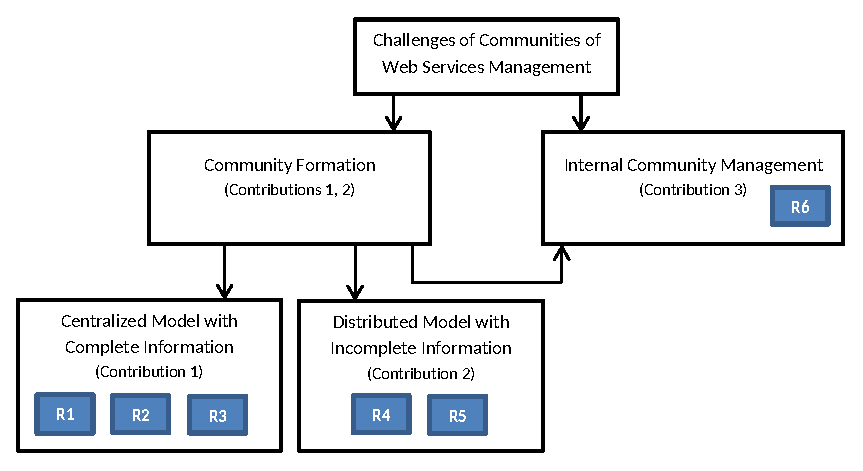
\includegraphics[width=6in]{Figures/model.eps}`
\caption{The Proposed Framework}
\label{fig_model}
\end{figure}

%\begin{figure}[!t]
%\centering
%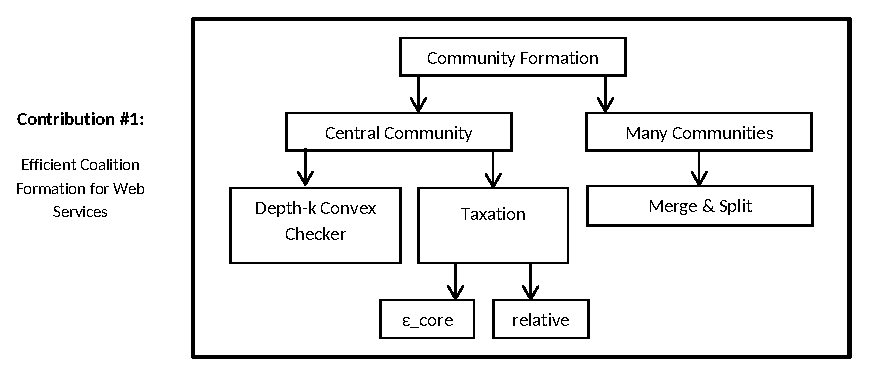
\includegraphics[width=6in]{Figures/c1.eps}`
%\caption{First contribution: Efficient Coalition Formation for Web Services}
%\label{fig_c1}
%\end{figure}
%
%\begin{figure}[!t]
%\centering
%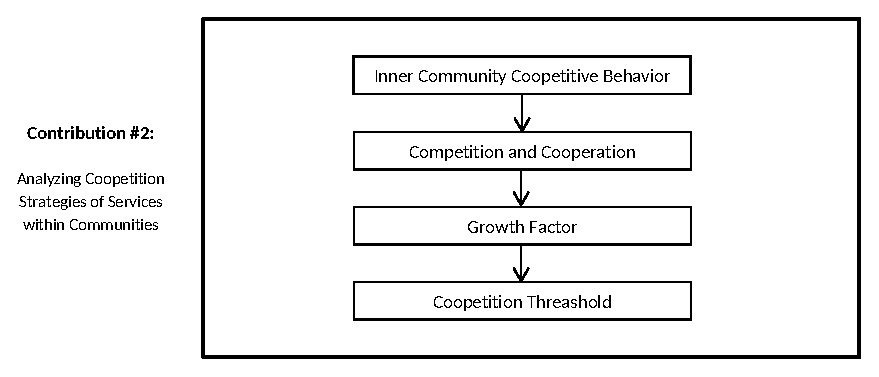
\includegraphics[width=6in]{Figures/c2.eps}`
%\caption{Second contribution: Analyzing Coopetition Strategies of Services within Communities}
%\label{fig_c2}
%\end{figure}
%
%\begin{figure}[!t]
%\centering
%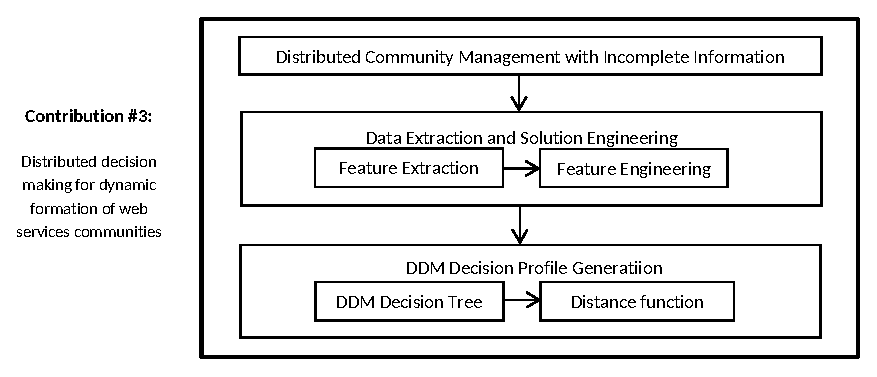
\includegraphics[width=6in]{Figures/c3.eps}`
%\caption{This contribution: Distributed decision making for dynamic formation of web services communities}
%\label{fig_c3}
%\end{figure}

Figure \ref{fig_model} highlights our contributions and proposed model for communities of web services formation and management.

\section{Thesis Organization}\label{sec:outline}
The rest of the proposal is organized as follows: We present in Chapter 2 the background needed for our research along with relevant related work. Chapter 3 provides an efficient method of coalition formation for web services. In Chapter 4 we discuss the cooperative behaviour within the communities of web services. Chapter 5 presents a distributed method of formation of web services communities. Finally in Chapter 6, we present our conclusion and future plan.


%%%%%%%%%%%%%%%%%%%%%%%%%%%%%%%%%%%%%%%%%%%%%%%%%%%%%%%%%%%%%%
%%%%%%%%%%%%%%%%%%%%%%%%%%%%%%%%%%%%%%%%%%%%%%%%%%%%%%%%%%%%%%

%
%\section{Context of Research}\label{sec:motivation_s}
%
%[seminar] Over the past years, online services have become part of many
%scalable business applications. The increasing reliance on
%web-based applications has significantly influenced the way web
%services are engineered.
%%Web services provide a set of stateless
%%software functions accessible at a network address over the web.
%%The recent developments are shifting web services from passive and
%%individual components to autonomous and group-based components
%%where interaction, composition, and cooperation are the key
%%challenges \cite{ICWS2011-1,SCC2011-1}. The main objective is to
%%achieve a seamless integration of business processes, applications
%%and web services. Delivering high quality services considering the
%%dynamic and unpredictable nature of the Internet is still a very
%%critical and challenging issue.
%%Typically, web services are business applications deployed as
%%autonomous and interoperable agents \cite{Alescio}. In fact, the
%%W3C consortium defines a web service as ``an abstract notion that
%%must be implemented by a concrete agent''. However, the web is
%%stocked with agent-based services that offer similar business
%%functionalities, which leads to service consumers having
%%difficulties in choosing the most appropriate agents to interact
%%with.
%The need for highly available and responsive services has called
%for grouping and collaborative mechanisms of loosely-coupled web
%services, particularly in business settings. The idea of grouping
%web services within communities and the way those communities are
%engineered so that web services can better collaborate have been
%proposed and investigated in
%\cite{DBLP:journals/ijebr/MaamarSTBB09,DBLP:journals/internet/BenatallahSD03,Rosario:2008:PQS:1512146.1512290}.
%Communities are virtual groups of web services having similar
%functionalities \cite{Zeng:2003:QDW:775152.775211,
%Paik:2005:TSS:2229263.2230038,Medjahed05adynamic,10.1109/ARES.2008.7},
%but probably different non-functional quality attributes, which
%form the QoS parameters.
%%When communities are used, users send
%%their requests to the masters of those communities, which are
%%responsible of managing the communities, forwarding the requests
%%to the suitable member web services and checking the credentials
%%of those members.
%Communities aim to provide higher service
%availability and performance than what individual web services can
%provide.
%%The high availability of services and the community
%%resilience to failure are guaranteed since web services can
%%cooperate and replace each other within the same community and
%%since there is no single point of failure in the communities
%%architecture.
%
%
%\section{Motivation and Research Objectives}\label{sec:motexample_s}
%
%Web service communities are dynamic by design
%\cite{DBLP:journals/ijebr/MaamarSTBB09}. In these communities, web
%services are modeled as intelligent autonomous agents, where they
%can adopt a strategy maximizing their payoff at any time. A web
%service can ask joining a community and has the right to leave it.
%Community managers can invite or ask a web service to leave in
%order to maximize the community profit. Users can simply stop
%sending requests to a web service which is not providing
%satisfactory services. Thus it is important to consider all the
%parties involved in the decision making process about the
%community management.
%
%In this research work, our first objective is to propose a
%cooperative model as game for the aggregation of web services
%within communities. The solution concepts of our cooperative game
%seeks to find efficient ways of forming coalitions (teams) of web
%services so that they can maximize their gain and payoff, and
%distribute the gain in a fair way among all the member services.
%Achieving Fairness when the gain is distributed among the
%community members is the main factor to keep the coalition stable
%as no web service will expect to gain better by deviating from the
%community. In other words, the coalition is made efficient if all
%the members are satisfied. We first propose a representation
%function for communities of web services based on their QoS
%attributes. By using this function, we can evaluate the $worth$ of
%each community of web services. When facing new membership
%requests, a typical community master checks whether the new
%coalition having the old and new set of web services will keep the
%community stable or not. The community master will reject the
%membership requests if it finds out that the new coalition would
%be unstable, preventing $any$ subset of web services from gaining
%significantly more by deviating from the community and joining
%other communities or forming new ones. The computation of
%solutions for cooperative games is combinatorial in nature and
%proven to be NP-complete \cite{Algorithmic}, making this
%computation impractical in real world applications. However, using
%the concepts of coalition stability, the second objective is to
%investigate approximation algorithms running in polynomial time
%providing web services and community masters with applicable and
%near-optimal decision making mechanisms.
%
%Within communities, services can exhibit competitive behavior as they provide the same functionalities and the number of users requests is finite.
%However, for the same reason of being functionally similar, services can cooperate with each other, for example to substitute each other in order to perform some sub-tasks.
%So as an extension of our work, we have proposed a framework in which services can opt for performing tasks if they feel they are capable enough
%or decide to cooperate by showing the availability to perform some sub-tasks.
%
%%We have implemented an online learning mechanism for services with different capabilities to learn over time which strategy to choose based on their own and other services status and capabilities. After establishing states of our model and observing convincing results from our learning method, we plan to extend the learning process using reinforcement learning (Q-learning) techniques.
%
%
%
%\indent To summarize, the main problems we aim to tackle in this
%thesis are the formation of stable and efficient coalitions
%maximizing web services and community revenue and the decision over the strategy to play about competing or cooperating.
%The main objectives are:
%\begin{itemize}
%\item To propose a cooperative model and analyze its solution
%concepts in order to address the problem of optimizing coalition
%formation for a stable community.
%
%\item To reduce the complexity of computing the solution concepts
%of the cooperative model tailored to the problem of communities of
%agent-based web services in order to make these solutions
%applicable in real world scenarios.
%
%\item To analyze the effect of different membership and taxation
%models that the master can apply to the members on the stability
%of the community.
%
%\item To investigate the impact of learning on individual and
%group decision making within the cooperative model of the
%community.
%
%\item To validate the proposed methods by extensive simulations
%and comparison with other similar proposals.
%\end{itemize}
%
%
%
%
%\section{Thesis Organization}\label{sec:outline_s}
%The rest of the thesis is organized as follows. We present in
%Chapter 111 the background needed for our research along
%with relevant related work. Chapter 222
%provides the problem statement and presents our solution model in
%two different scenarios with some preliminary results. Finally, in
%Chapter 333, we present our conclusion,
%future plan, and the timetable of our research.
%
%
%
